%!TEX root = ../documentation.tex



%% SUBSECTION
\subsection{Rational Unified Process}
\label{sec:zusammenarbeit:rup}

Der \emph{Rational Unified Process (RUP)} ist zum einen ein Vorgehensmodell, zum anderen auch die zugehörigen Entwicklungswerkzeuge, die von IBM vertrieben werden. Entstanden ist RUP als Kombination der Prozesse der Firmen \emph{Rational} und \emph{Objectory}. Kombiniert werden dabei ein iterativer, inkrementeller Softwareprozess mit architekturzentrierter Vorgehensweise und die objektorientierte Darstellung, meist in Form von Use-Case-Diagrammen. \cite[49,50]{Hughes:2015:Agile:05}
\\
Im Gegensatz zu z. B. dem Wasserfallmodell überschneiden sich die einzelnen Phasen bei RUP und unterscheiden sich vor allem in ihrer Intensität voneinander in zeitlicher Hinsicht. Abbildung \ref{fig:rup} veranschaulicht hierbei die zwei Dimensionen von RUP. Die vier Phasen sind dabei \emph{Konzept}, \emph{Entwurf}, \emph{Implementierung} und \emph{Produktübergabe}. Zu erkennen ist, dass die Implementierung bereits während der Konzeptphase beginnt und die Analyse und Design auch während der Implementierung noch aktiv ist. Dadurch kann auf Anforderungsänderungen im Projektverlauf eingegangen werden. Zudem findet eine deutlich ausgeprägtere Kommunikation zwischen den verschiedenen Teams statt \cite[6,7]{Versteegen:2000:Projektmanagement:25}. 
\\
Im Unterschied zu z. B. Scrum ist RUP ein kommerzielles Produkt. Es kann ohne Anpassungen direkt verwendet werden, bietet aber auch die Möglichkeit der Erweiterung und Anpassung \cite[31]{Kruchten:1999:Der-Rational:67}.




\begin{figure}
\centering
    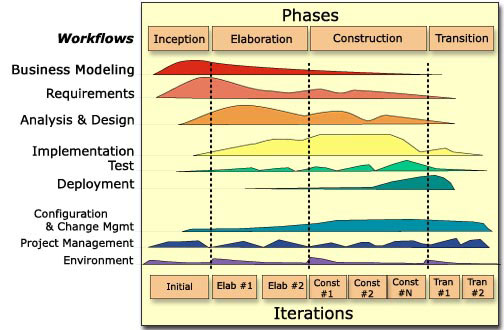
\includegraphics[width=0.7\textwidth, height=0.7\textheight,keepaspectratio]{Two-Dimensions-of-the-RUP} 
    \caption{Dimensionen von RUP. Übernommen von \cite{Kruchten:2000:The-Rational:47}}
    \label{fig:rup}
\end{figure}

%% SUBSECTION
\subsection{Scrum}
\label{sec:zusammenarbeit:scrum}

Scrum ist ein, vor allem von \emph{Ken Schwaber} und \emph{Jeff Sutherland} entwickeltes Vorgehensmodell, das der agilen Software-Entwicklung zugerechnet werden kann. Es wird seit den 1990er Jahren entwickelt und findet seitdem eine steigende Verbreitung \cite[1]{Schwaber:2020:The-Scrum:15} \cite{research:2018:Scrum:67}. Einer der Kerngedanken von Scrum ist die selbstständige Arbeit der Mitarbeiterinnen und Mitarbeitern und das regelmäßige Reflektieren und Anpassen von Methoden und Vorgehensweisen um möglichst immer optimale Resultate zu erzielen. Um das zu erreichen teilt Scrum komplexe Probleme in kleinere Probleme auf, die für sich erarbeitet und bewertet werden können \cite[3]{Schwaber:2020:The-Scrum:15}.
\\
Dabei gibt Scrum keine detaillierten Anweisungen vor, wie etwas zu tun ist, sondern lediglich einen Rahmen, der dafür essentiell ist. Innerhalb dieser Freiheit soll die Expertise der Mitarbeiterinnen und Mitarbeitern dafür sorgen, dass die nötigen Dinge getan werden. \cite{Schwaber:2020:The-Scrum:15}
\\
Die enge Zusammenarbeit, sowohl innerhalb des Teams als auch mit Kundinnen und Kunden ist hier stark ausgeprägt. Während sich z. B. das V-Modell stärker auf die Übergabe von Dokumenten verlässt, steht hier ein häufiger Kontakt im Fokus \cite{Shiklo:2019:8-Vorgehensmodelle:12}.
Im wesentlichen gibt es nur drei Artefakte bei Scrum, \emph{Product Backlog}, \emph{Sprint Backlog} und \emph{Increment} \cite[10-12]{Schwaber:2020:The-Scrum:15}.


%% SUBSECTION
\subsection{Vergleich der vier Vorgehensmodelle}

Bei einem Vergleich der vier Modelle lässt sich eine Einteilung in zwei Dimensionen vornehmen. Wie Abbildung \ref{fig:modelleEinor} zeigt kann ein Modell einerseits als formell oder informell eingeordnet werden, andererseits kann in sequentielle und evolutionäre Modelle unterschieden werden. Sowohl das Wasserfallmodell als auch das darauf aufbauende V-Modell sind stark formell aufgebaut und stützen sich auf eine extensive Dokumentation, die bei der sequentiellen Abarbeitung des Entstehungsprozesses den Rahmen bildet. Die Zusammenarbeit findet hier primär über diese Artefakte statt, z. B. auch beim Übergang von Designphase zu Implementierungsphase. 
\\
Bei Scrum stehen deutlich weniger formelle Artefakte im Vordergrund, sondern die direkte Zusammenarbeit verschiedener Spezialistinnen und Spezialisten. Auch bei der Zusammenarbeit mit Kundinnen oder Kunden ist diese stärker ausgeprägt und es werden im Sinne einer evolutionären Entwicklung auch unvollständige Produktstände zum Testen an diese weitergegeben. RUP stellt einen Mittelweg dar, da zwar ebenfalls evolutionär vorgegangen wird, aber trotzdem noch ein stärkerer formeller Fokus als bei Scrum im Vordergrund steht. %\cite{Shiklo:2019:8-Vorgehensmodelle:12}

\begin{figure}
\centering
    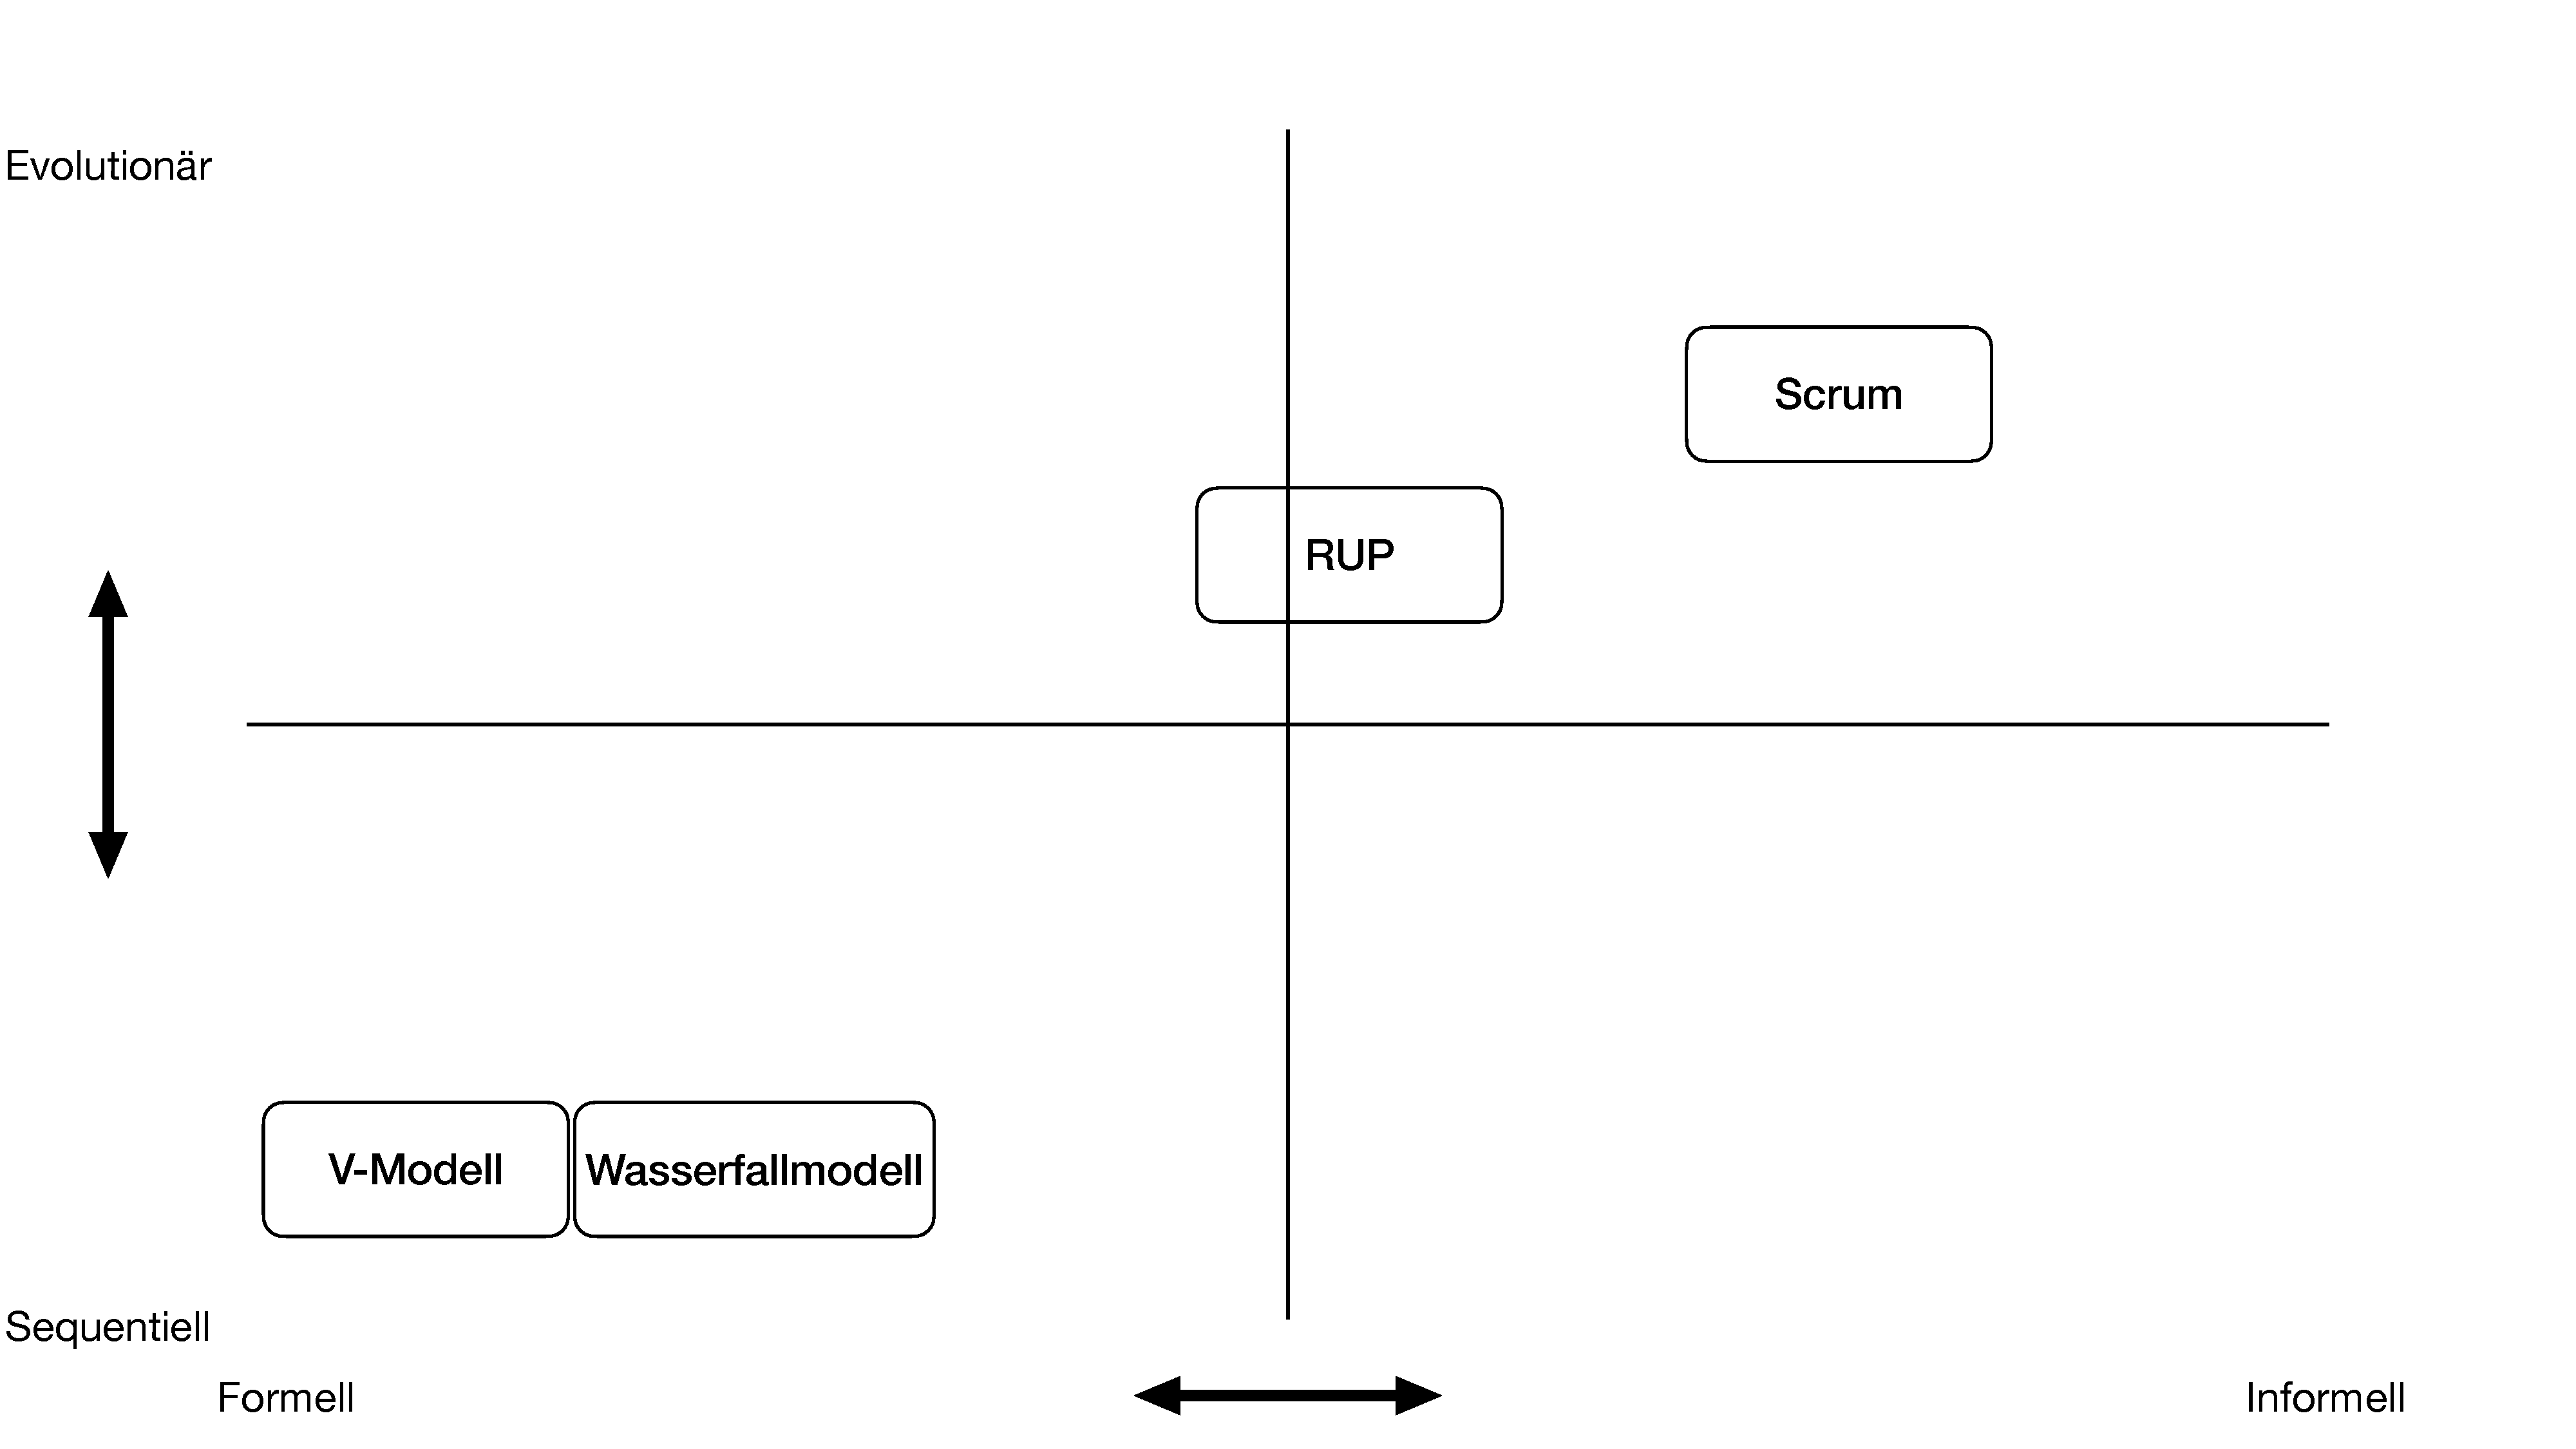
\includegraphics[width=0.7\textwidth, height=0.7\textheight,keepaspectratio]{EinordnungModelle} 
    \caption{Einordnung von Vorgehensmodellen. Angepasst nach \cite{Shiklo:2019:8-Vorgehensmodelle:12}}
    \label{fig:modelleEinor}
\end{figure}

%Unterschiede zwischen den einzelnen Verfahrensmodellen bestehen zum Beispiel darin, wie das jeweilige Modell aufgebaut ist. Jedes Modell ist linear oder iterativ strukturiert. Bei RUP besteht die Besonderheit, dass es eine Kombination aus beidem ist. Scrum ist iterativ aufgebaut, wohingegen das V-Modell und das Wasserfallmodell eine lineare Struktur besitzen, also alle Phasen nacheinander ablaufen. Beim Wasserfall- und V-Modell ist durch die lineare Vorgehensweise eine bessere Planung verschiedener Faktoren, wie Kosten, Zeit und Mitarbeiter gegeben als bei Scrum. (vgl. Shiklo) Außerdem sind sie durch die lineare Struktur grundsätzlich einfach und einfacher zu implementieren als Scrum und RUP. Des Weiteren können sie im Nachhinein auch einfacher verwaltet werden. (vgl. Shiklo) 
%Im Vergleich zum Wasserfallmodell, bei welchem die Dokumentation eine wichtige Rolle spielt, tritt diese bei Scrum in den Hintergrund. Hier stehen die Testaktivitäten im Fokus. (vgl. Shiklo) Das V-Modell ist ein qualitativ hochwertiges Modell und erkennt Fehler und Risiken frühzeitig, allerdings ist es auch das teuerste und zeitintensivste Modell. Außerdem ist es wie sehr unflexibel was Anforderungsänderungen während des Prozesses betrifft. Der letzte Punkt trifft auch auf das Wasserfallmodell zu. (vgl. Shiklo)
%Ein weiterer wichtiger Punkt hinsichtlich der Unterschiede in der Zusammenarbeit betrifft die Einbeziehung der Kunden und Kundinnen. Das Beziehungsgeflecht zwischen den Mitarbeitenden und dem Kunden oder der Kundin kann in Verfahrensmodellen informell oder formell konzipiert sein. Auch die Verfahrensmodelle, welche in dieser Arbeit vorgestellt wurden, unterscheiden sich in den genannten Punkten. So sind das Wasserfallmodell und das V-Modell stark formell ausgeprägt, wohingegen RUP schon deutlich informeller gestaltet ist und Srum eine starke informelle Ausprägung besitzt. Das bedeutet, dass der Kunde oder die Kundin beim RUP und vor allem bei Scrum intensiv in die Projektentwicklung eingebunden ist. Daraus kann geschlossen werden, dass sich auch die Zusammenarbeit innerhalb des Teams dahingehend unterscheidet, inwieweit neben den Teammitgliedern mit den Kunden und Kundinnen zusammengearbeitet wird. So werden beim V-Modell und beim Wasserfallmodell alle Wünsche und Anforderungen zu Beginn des Projekts bereits festgelegt und können nicht wie bei den anderen beiden Modellen vor der nächsten Iteration auf verändernde Kundenwünsche eingehen.



Ein weiterer wichtiger Unterschied zwischen den vier Vorgehensmodellen besteht darin, in welchen Bereichen das jeweilige Modell am geeignetsten ist. Das V-Modell und Wasserfallmodell eignen sich durch ihren Schwerpunkt auf eine präzise, gut dokumentierte Vorgehensweise z. B. für Anwendungsbereiche, in denen ebenfalls ein präzises Vorgehen unabdingbar ist. Shiklo \cite{Shiklo:2019:8-Vorgehensmodelle:12} nennt an dieser Stelle Softwareunternehmen im Bereich der Medizin oder dem Luftverkehr sowie staatliche Projekte, da hier vorhersehbare Projektpläne und Budgets mit einer strengen Kontrolle erforderlich sind. 
\\
Evolutionäre Vorgehensmodelle, wie etwa RUP können optimal für größere Projekte eingesetzt werden, bieten im Vergleich zu den sequentiellen Modellen aber bessere Möglichkeiten bei Anforderungsänderungen im Projektverlauf. Dabei ist RUP erst ab einer gewissen Projektgröße sinnvoll einzusetzen, da eine Vielzahl an Rollen erfüllt werden müssen. Scholz \cite[150]{Scholz:2005:Softwareentwicklung:09} nennt eine Teamgröße mit mehr als zehn Personen, mehr als 30 Rollen und über 100 verschiedene Artefakttypen. 
\\
Im Gegensatz dazu ist Scrum, als rein agiles Modell, vor allem für kleine Teams geeignet. Dies wird unterstützt durch eine Untersuchung, dass kleinere Teams bessere Leistung erbringen \cite{Hackman:1970:Effects:85}. Das kann z. B. bei Start-Up-Unternehmen der Fall sein, bei denen die Kundeneinbeziehung auch stärker im Vordergrund steht. Aber auch größere Projekte können mithilfe von Scrum bewältigt werden, wenn diese in kleinere Teilprojekte aufgeteilt werden können. Hier hat sich der Begriff des \emph{Scrum-of-Scrums} entwickelt, wobei die einzelnen Scrum-Teams einen Vertreter wählen, der wiederum Teil der übergeordneten Scrum-Teams ist \cite[227]{Dalton:2019:Great:62}.
%RUP eignet sich zum Beispiel für Use-Case-Projekte oder, wenn qualitativ hochwertige Software schnell zur Verfügung stehen soll. Im Vergleich zu RUP ist Scrum ebenfalls iterativ strukturiert. Anders als RUP handelt es sich bei Scrum jedoch um ein rein agiles Modell, das laut Shiklo () den Vorteil hat, dass es schneller und anpassungsfähiger ist. Scrum kann also auch bei größeren Projekten Anwendung finden, wenn diese in kleinere Teilschritte gegliedert werden können. Außerdem ist Scrum ideal für Start-Up-Unternehmen, da die Kundenbeziehung und -einbeziehung hier im Vordergrund steht. (vgl. Shiklo)
%Wie herausgearbeitet werden konnte, unterscheidet sich die Zusammenarbeit innerhalb der einzelnen Modelle im Hinblick auf die Kundenbeteiligung, ob es sich um ein lineares oder iteratives Modell handelt und worauf der Fokus im Projektprozess gelegt wird. Jedes Modell besitzt gegenüber den anderen Modellen Vor- und auch Nachteile, weswegen es wichtig ist, individuell je nach Unternehmens- und Projektart zu entscheiden, welches Modell am geeignetsten erscheint. 
%\todo{auskommentiert wieder einbauen?!}
%Damit eine Zusammenarbeit im Team funktioniert, können wie beschrieben die Verfahrensmodelle eingesetzt werden. Auf der anderen Seite hängt ein Gelingen auch davon ab, wie das Projekt geplant wird. Hier spielt der Projektleiter oder die Projektleiterin eine entscheidende Rolle. Laut Verstaagen (S. 163) ist es wichtig, genau zu planen, wann wie viele und welche Mitarbeitenden eingeplant werden, damit jeder und jede eine konkrete Aufgabe hat und keine Verwirrungen und Unstimmigkeiten entstehen. 
\\
Allen genannten Modellen gemein ist, dass sie in Bezug auf die konkrete Zusammenarbeit relativ abstrakt bleiben. Welche Strategien und Werkzeuge können z. B. in der Phase der Implementierung helfen, Probleme zu vermeiden? Darauf geht das folgende Kapitel näher ein.



